
We are going to discuss about two tools for cryptographic protocol verification: \href{https://prosecco.gforge.inria.fr/personal/bblanche/proverif/}{Proverif} and \href{https://tamarin-prover.github.io/}{Tamarin-Prover} . Tamarin-Prover will also be referred to as Tamarin for brevity.

First of all, let us consider the different types of approaches to security protocol analysis. The two categories of techniques are shown in figure \ref{fig:symbolic-computational-model} and we will proceed examining them.

\begin{figure}[!h]
    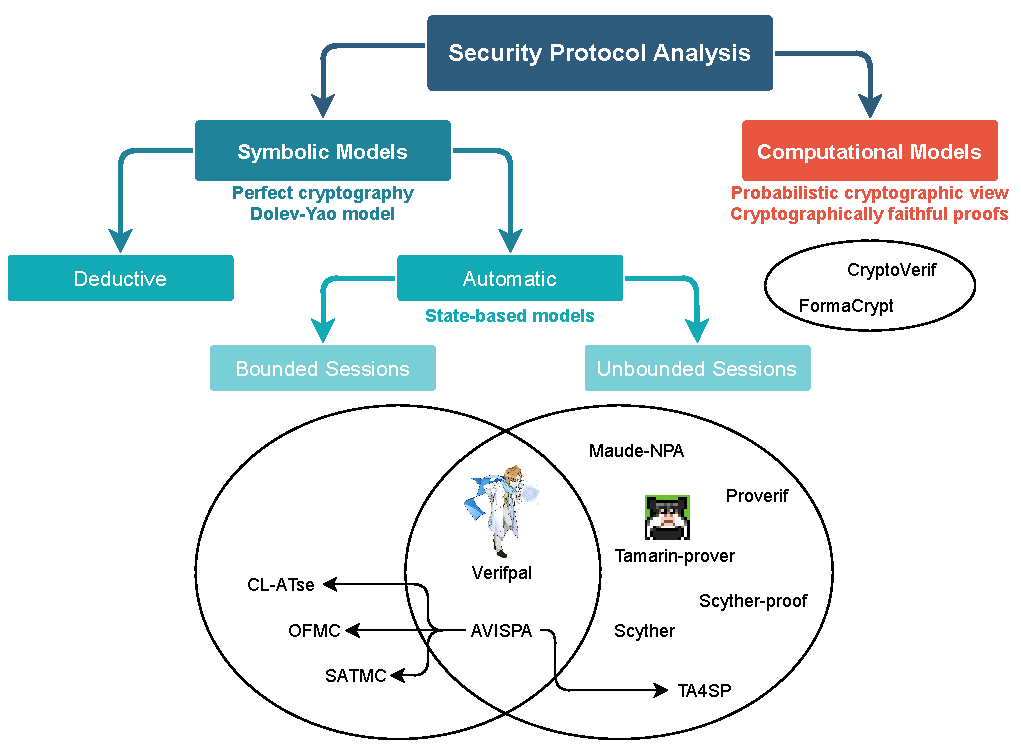
\includegraphics[scale=0.9]{symbolic-computational-model}
    \centering
    \label{fig:symbolic-computational-model}
    \caption{Symbolic and computational models}
\end{figure}

In the \textit{symbolic model} (often called Dolev-Yao model) \cite{Dolev-Yao}, the cryptographic primitives are considered as black-box and are represented using function symbols, the messages are terms and the adversary can only use defined primitives. An important aspect to note of this model is that it assumes \textbf{perfect cryptography}. As an example, consider the case in which there are two function symbols (\textbf{enc} and \textbf{dec}, used to encrypt and decrypt), a message \textit{m} and a key \textit{k} and the following equality is defined:

\begin{equation}
\mbox{dec}\left(\mbox{enc}\left(m, k\right), k\right) = m
\end{equation}

Following from the equation $-$ and considering the perfect cryptography assumption $-$ it is possible to decrypt $\mbox{enc}\left(m, k\right)$ if and only if \textit{k} is known \cite{SymbolicComputationalBlanchet}.


In the \textit{computational model} the messages are bitstrings, the cryptographic primitives are functions from bitstrings to bitstrings and the attacker is modeled as a probabilistic Turing machine.
A security property in this model is considered to hold when the probability that it does \textit{not} hold is negligible. For instance, the previously discussed shared-key encryption can be modeled using the same equalities, but the security of encryption is expressed by stating that the attacker has an insignificant probability of breaking the primitive (e.g. decrypting the message without having the key). Security proofs using this model are usually stronger, however this comes to the cost of long, difficult, tedious and highly error prone proofs (as stated by INRIA researchers \cite{ComputationalAnalysisCryptoSystemsINRIA}). Finally, as pointed to by Blanchet \cite{SymbolicComputationalBlanchet}, the computational model is indeed just a \textit{model} and ignores many aspects of reality and potential attacks, e.g. faulty attacks like the RSA one \cite{RSAFaultAttack}. 

Both Proverif and Tamarin employ a symbolic model. This makes it possible to automate proofs when given a set of primitives, a protocol model and a set of security properties. Note that termination is still not always guaranteed \footnote{It actually depends on the tool. Proverif proofs always terminate, but they might terminate with an inconclusive result, while Tamarin may simply not terminate without ever giving a result. More details about this problem will be discussed later.}. % TODO: discuss non termination issues!!

\section{Proverif}
% TODO

\section{Tamarin}
In this section we will see an overview of Tamarin foundations and internal reasoning.
For a more in-depth description and further information, see the Tamarin foundations paper \cite{TamarinFoundations} or the extended foundations paper \cite{TamarinFoundationsExtended}.

\subsection{High level view}
First of all, let's have a look at an high level picture of Tamarin.

The security property model of Tamarin is based on multiset rewriting rules to specify protocols and adversary capabilities, a guarded fragment \footnote{Only a few examples of formulas respecting the guarded fragment of first order logic used by Tamarin will be given in the next subsections. See \cite{FragmentFirstOrderLogicPaper} for a rigorous definition from a mathematical point of view.} of first order logic to specify security properties \footnote{Security properties in Tamarin will also be referred to as \textit{lemmas}.} and functions and equational theories to model the algebraic properties of cryptographic protocols \cite{TamarinFoundations}. % TODO: show a few examples of first order logic formulas respecting the guarded fragment!!

Given the rewriting rules, security properties and equational theories, Tamarin uses a novel constraint-solving algorithm which tries to validate or falsify lemmas.

Tamarin also offers builtin equational theories \cite{TamarinProverManual}. A brief overview will be given in subsection \ref{sub:Builtin-equational-theories}.

\subsection{Transition rules}
\label{sub:Transition-rules}
As reported earlier, multiset rewriting rules are used to specify adversary capabilities and protocols. More precisely, a \textit{set} of \textit{labeled} multiset rewriting rules are used.

The components for these multisets are the following:

\begin{description}[style=nextline]
    \item[Terms] which can be essentially thought of as messages. Terms can be of three different sorts. The more general sort is the \textit{msg} sort, which has two incomparable subsorts \textit{fresh} and \textit{pub} for fresh and public names;
    \item[Facts] which model information in the protocol. Facts have an arity, can be linear or persistent and are composed by terms. By convention, they always start with a capital letter;
    \item[Special facts] Four facts are reserved and are used to model the freshness of a message $t$ ($\mbox{\textbf{Fr}}\left(t\right)$), a message $t$ coming from the public channel ($\mbox{\textbf{In}}\left(t\right)$), a message $t$ to be output to the public channel ($\mbox{\textbf{Out}}\left(t\right)$) and knowledge of a certain message $t$ from the attacker ($\mbox{\textbf{K}}\left(t\right)$);
    \item[State of the system] The state of the system is represented using a finite \textit{multiset} of facts;
    \item[Transition rules] A multiset of transition rules defines the possible transitions from one state to another one. Transitions are denoted with the following syntax
    \begin{equation}
        L \msrewrite{A} R
    \end{equation}
    where $L, A$ and $R$ are multisets of facts.
\end{description}

Let us examine an informal description of transitions.

\begin{itemize}
    \item{Let $S$ be the current state of the system}
    \item{Let $\msrnolabel{L}{R}$ be a transition rule. Note that this is a \textit{multiset rewriting rule} without a \textit{label};}
    \item{Let $\msrnolabel{l}{r}$ be a ground instance of the rule (i.e. no variables are present in the multisets);}
    \item{If we apply $\msrnolabel{l}{r}$ to our state $S$ we reach a new state, defined by the following equation:
    \begin{equation}
        S \msrsetminus l \msrcup r
    \end{equation}
    We use $\msrsetminus$ and $\msrcup$ to define difference and union over multisets, respectively;}
    \item{When we use labelled multiset rewriting rules, such as $\msr{l}{a}{r}$, we also add facts from $a$ to the \textit{trace} of the execution.}
\end{itemize}

Tamarin defines two transition rules


\subsection{Builtin equational theories}
\label{sub:Builtin-equational-theories}
A brief list of Tamarin built-ins is given below: \footnote{Only the builtin theories considered relevant and those used in the analysis will be described here. The full list is available in the Tamarin manual. \cite{TamarinProverManual}}

\begin{description}[style=nextline]
    \item[hashing] defines a perfect hash function \textbf{h/1} \footnote{The writing \textbf{f/x} indicates that the function \textbf{f} has arity \textbf{x}.};
    \item[asymmetric-encryption] models a public key encryption scheme. It defines the following symbols:
    
    \begin{itemize}
        \item{\textbf{aenc/2}, used to model the encryption of a message with a public key}
        \item{\textbf{adec/2}, used to model the decryption of an encrypted message with a private key}
        \item{\textbf{pk/1}, used to derive a public key from a private key}
    \end{itemize}

    Functions are related by the equation \textbf{adec(aenc(msg, pk(sk)), sk) = msg};

    \item[diffie-hellman] models Diffie-Hellman groups. It defines the following symbols:
    
    \begin{itemize}
        \item{\textbf{inv/1}, models the inverse of an element}
        \item{\textbf{1/0}, models the neutral element}
        \item{\textbf{\textasciicircum} and \textbf{*} symbols, models exponentiation and multiplication respectively}
    \end{itemize}

    The equational theory for this builtin is actually quite complex. For the sake of completeness, these are the related equations:
    \begin{itemize}
        \item{(x \textasciicircum y) \textasciicircum z = x \textasciicircum (y * z)}
        \item{x \textasciicircum 1 = x}
        \item{x * y = y * x}
        \item{(x * y) * z = x * (y * z)}
        \item{x * 1 = x}
        \item{x * inv(x) = 1}
    \end{itemize}
    % TODO: parla ancora un po' di quanto sia figo Tamarin che ha DH builtin!
\end{description}

\section{Comparison of Proverif and Tamarin}